\documentclass[a4paper,11pt]{article}


\usepackage{amsmath,amsfonts,amsthm,a4wide}
\usepackage{graphicx}
\usepackage[super]{nth}
\usepackage{mathtools}


\begin{document}
\begin{center}
University of Toronto at Scarborough\\[0.1in]
{\bf CSCC73H3 Algorithm Design and Analysis, FALL 2018} \\[0.1in]
{\large{\bf Assignment No.5: Dynamic Programming and Network Flow}}\\[0.1in]
{\bf DUE:} November 8, 2018, at 11:59 pm
\end{center}


\vspace{0.1in}
\noindent
{\bf Student ID:} 1005642654 \\[0.15in]
{\bf Student Name:} KyooSik Lee
\vspace{0.3in}

\vspace{0.3in}
\begin{enumerate}

\item

On Assignment No.6

\item 

{\bf Description}

\begin{enumerate}

	\item
	The statement is false. The counter example is below.

	\begin{figure}[hbt]
		\centering
		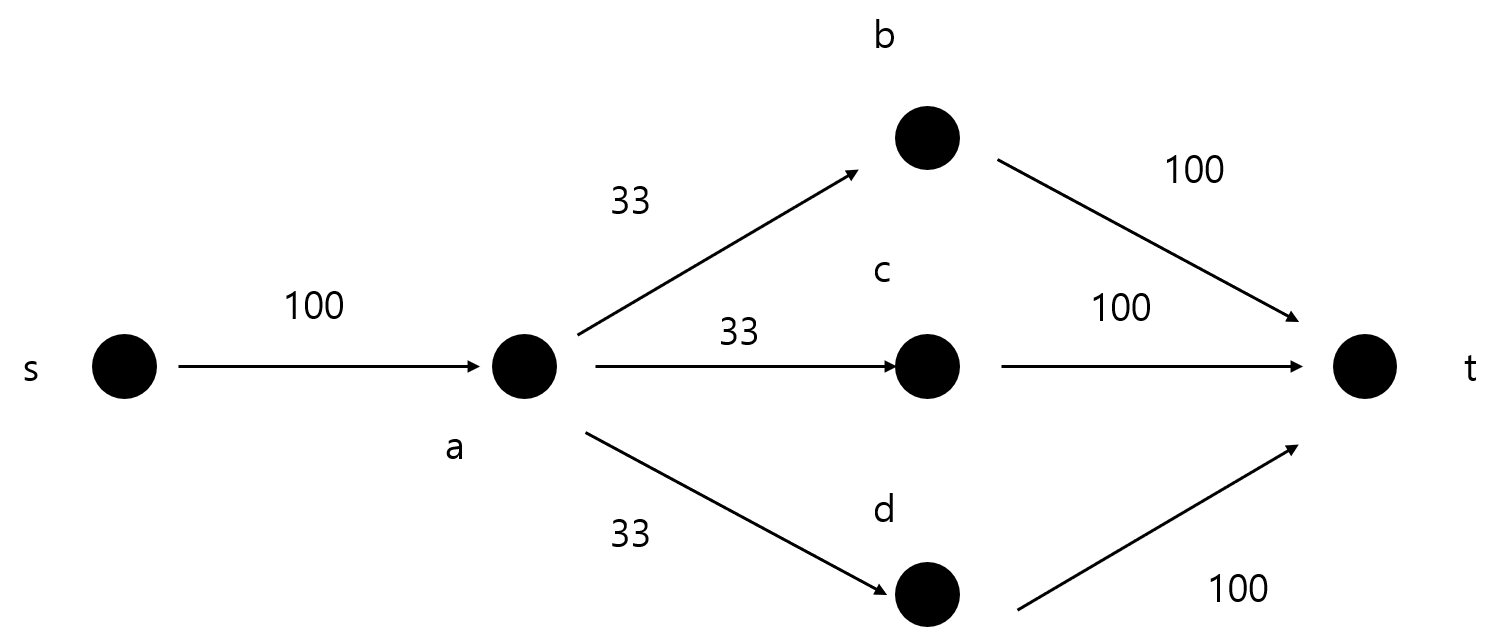
\includegraphics[scale=0.4]{figure1.png}
		\caption{Original Network $G$}
	\end{figure}

	At Figure 1 the $minimum$ $s-t$ $cut$ is s and a. After adding 1 to each edges, the graph follows.

	\begin{figure}[hbt]
		\centering
		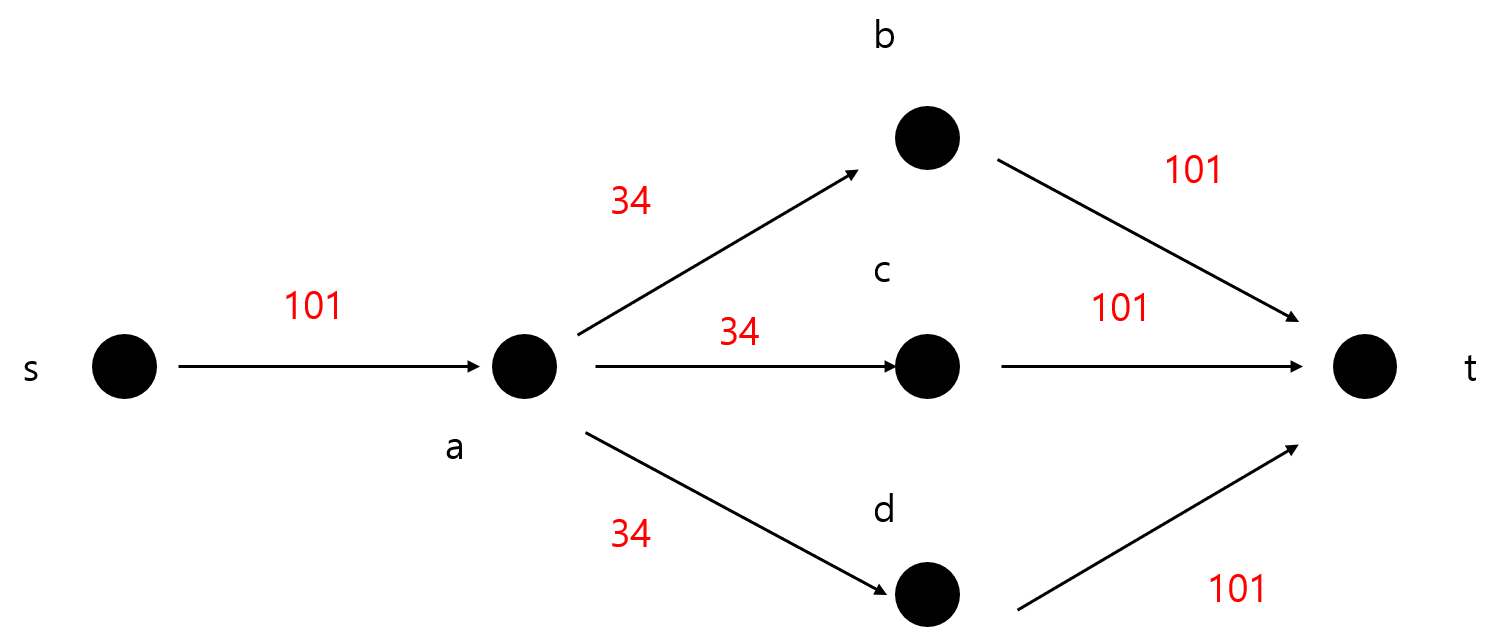
\includegraphics[scale=0.4]{figure2.png}
		\caption{One Added Network $G'$}
	\end{figure}

	We can see that now the $minimum$ $s-t$ $cut$ is only s.

	By showing counterexample, the statement is false.


	\item
	$(u,v)$ is increased by k. Then use the max flow algorithm covered in class. This is done by finding path from $s$ to $u$ and a path from $v$ to $t$. 
	Finding path could be done by DFS, which has complexity of $O(V+E)$. Therefore the algorithm takes $O(V+E)$ time complexity.
		\begin{figure}[hbt]
		\centering
		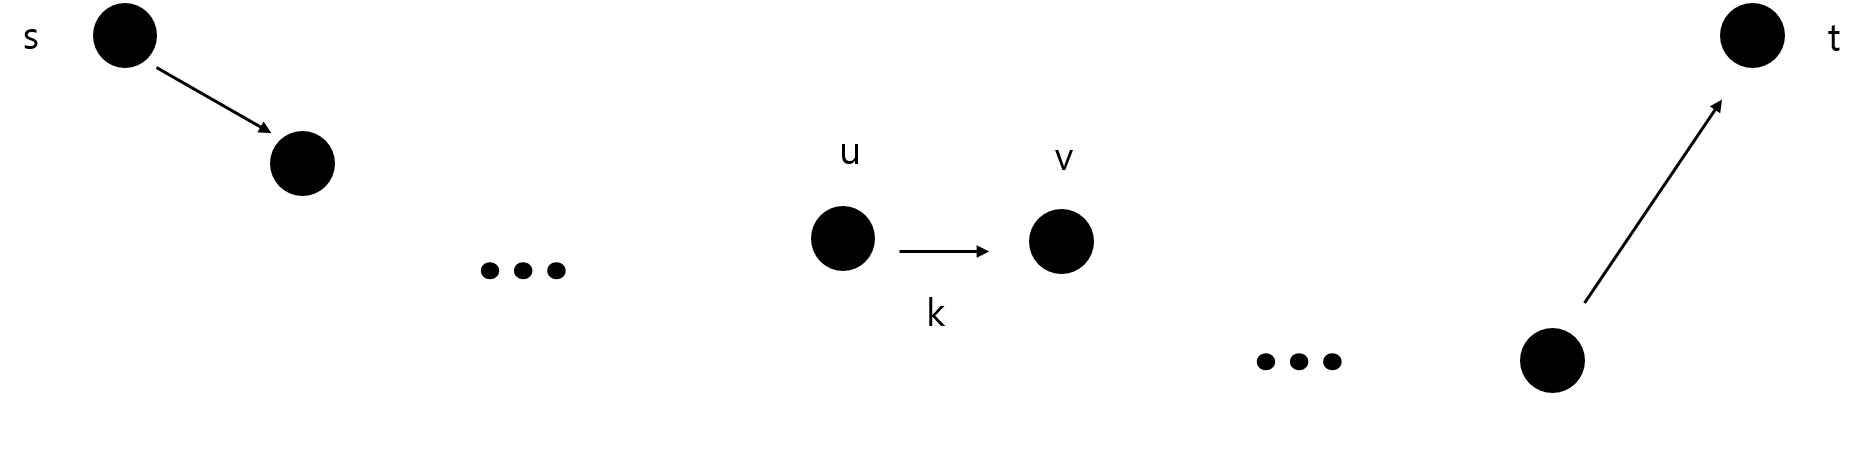
\includegraphics[scale=0.4]{figure3.png}
		\caption{k added Network}
		\end{figure}

	This is enough because if the addition of $k$ only affects this one path $p$.
	
	{\bf Proof}

	My algorithm will add residual graph by any value that $p$ allowed. Then any other possible path from $s$ to $p$ on the newly edited graph should use the reverse direction of $p$. If not, it contradicts that the original network is maximum network flow.
		\begin{figure}[hbt]
		\centering
		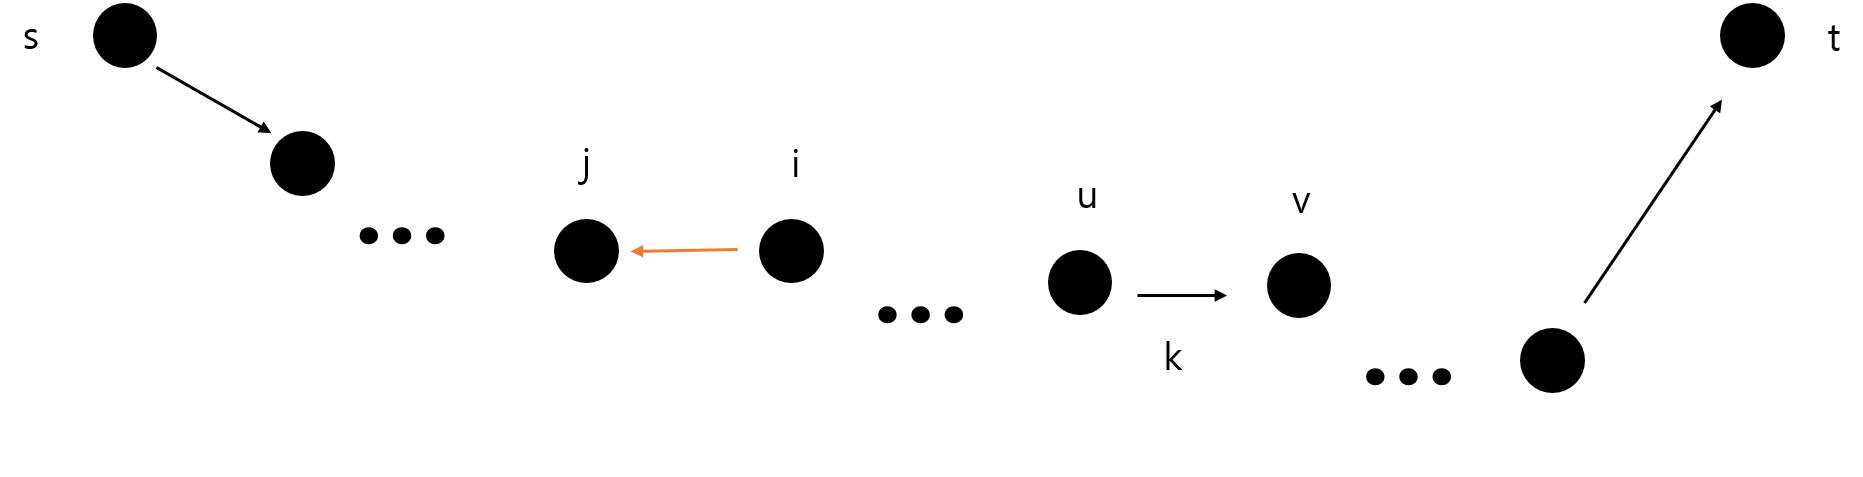
\includegraphics[scale=0.4]{figure4.png}
		\caption{Network with i j}
	\end{figure}
	If we use any residual direction path of reverse path $p$, let's call that edge $(i, j)$. Both $i$ and $j$ is in path $p$. Because there is a path from $s$ to $i$ to $j$ to $t$(this is what we have assumed). Then this means at the original network, there is a path from $s$ to $i$ to $t$ or $s$ to $j$ to $t$. This depends on the position of edge $(u,v)$. If it was before $(j,i)$ on $p$, it means that the original network has a path from $s$ to $i$ to $t$ and contradiction rises. Otherwise if the $(u,v)$ was after $(j,i)$, then there was path from $s$ to $j$ to $t$. This also rise contradiction.

\end{enumerate}
\pagebreak
\item{\bf Description}

First set up a network  by Figure5.

\begin{figure}[hbt]
\centering
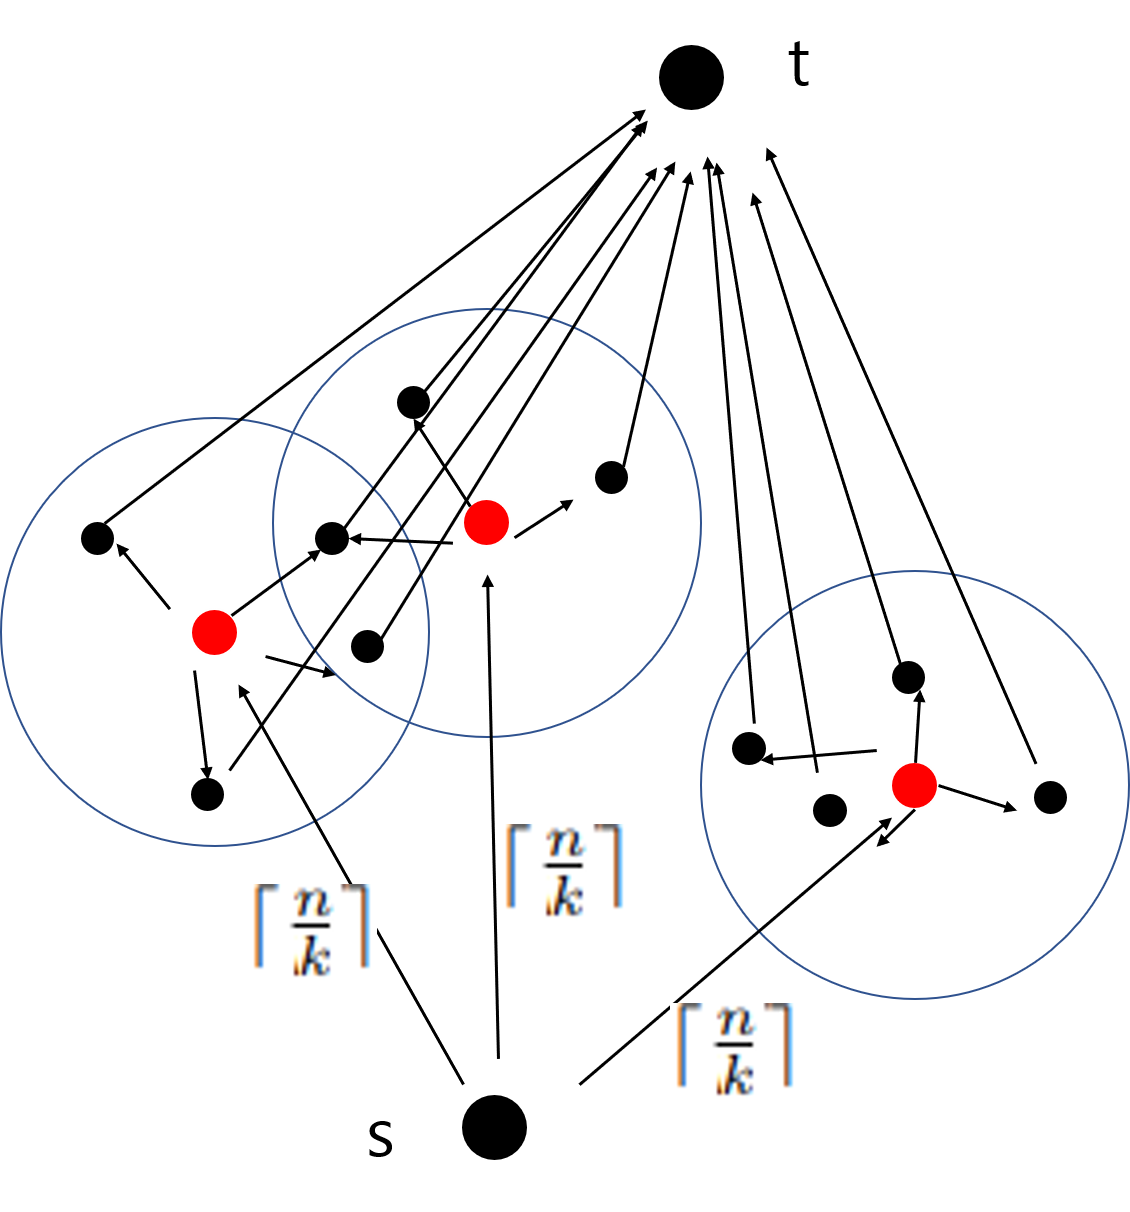
\includegraphics[scale=0.4]{figure5.png}
\caption{Network Flow of School and Houses}
\end{figure}

The boundary represents the school catchment area which is 1 km radius circle. The middle of the circle is school. The small circles represent houses of students.

We set up a network by adding $\lceil \frac{n}{k}\rceil$ to every edge from $s$ to each school. The school has edge 1 to every houses. 
The houses have edge 1 to $t$.

Then we do the maximum network flow algorithm covered in class.


\end{enumerate}







\end{document}
